% !TEX TS-program = pdflatex
% !TEX encoding = UTF-8 Unicode

\documentclass[a4paper, titlepage=false, parskip=full-, 10pt]{scrartcl}

\usepackage[utf8]{inputenc}
\usepackage[T1]{fontenc}
\usepackage[english, ngerman]{babel}
\usepackage{babelbib}
\usepackage{hyperref}
\usepackage{listings}
\usepackage{framed}
\usepackage{color}
\usepackage{graphicx}
\usepackage[normalem]{ulem}
\usepackage{cancel}
\usepackage{amsmath}
\usepackage{amssymb}
\usepackage{amsthm}
\usepackage{algorithm}
\usepackage{algorithmic}
\usepackage{geometry}
\usepackage{subfigure}
\geometry{a4paper, top=20mm, left=35mm, right=25mm, bottom=40mm}

\newcounter{tasknbr}
\setcounter{tasknbr}{1}
\newenvironment{task}[1]{{\bf Aufgabe \arabic {tasknbr}\stepcounter{tasknbr}} (#1):\begin{enumerate}}{\end{enumerate}}
\newcommand{\subtask}[1]{\item[#1)]}

% Listings -----------------------------------------------------------------------------
\definecolor{red}{rgb}{.8,.1,.2}
\definecolor{blue}{rgb}{.2,.3,.7}
\definecolor{lightyellow}{rgb}{1.,1.,.97}
\definecolor{gray}{rgb}{.7,.7,.7}
\definecolor{darkgreen}{rgb}{0,.5,.1}
\definecolor{darkyellow}{rgb}{1.,.7,.3}
\lstloadlanguages{C++,[Objective]C,Java}
\lstset{
escapeinside={§§}{§§},
basicstyle=\ttfamily\footnotesize\mdseries,
columns=fullflexible, % typewriter font look better with fullflex
keywordstyle=\bfseries\color{blue},
% identifierstyle=\bfseries,
commentstyle=\color{darkgreen},      
stringstyle=\color{red},
numbers=left,
numberstyle=\ttfamily\scriptsize\color{gray},
% stepnumber=5,
% numberfirstline=true,
breaklines=true,
% prebreak=\\,
showstringspaces=false,
tabsize=4,
captionpos=b,
% framexrightmargin=-.2\textwidth,
float=htb,
frame=tb,
frameshape={RYR}{y}{y}{RYR},
rulecolor=\color{black},
xleftmargin=15pt,
xrightmargin=4pt,
aboveskip=\bigskipamount,
belowskip=\bigskipamount,
backgroundcolor=\color{lightyellow},
extendedchars=true,
belowcaptionskip=15pt}

%% Enter current values here: %%
\newcommand{\lecture}{Algorithmische Geometrie SS15}
\newcommand{\tutor}{}
\newcommand{\assignmentnbr}{9}
\newcommand{\students}{Julius Auer, Alexa Schlegel}
%%-------------------------------------%%

\begin{document}  
{\small \textsl{\lecture \hfill \tutor}}
\hrule
\begin{center}
\textbf{Übungsblatt \assignmentnbr}\\
[\bigskipamount]
{\small \students}
\end{center}
\hrule

\begin{task}{Platonische Körper}
\item[]
Platonische Körper sind volkommen regelmäßige konvexe Polyeder. Polyeder sind dreidimensionale Körper, die von Polygonen (Vielecken) als Seitenflächen begrenzt sind.


\subtask{a}
Beweisen Sie, dass es in 3 Dimensionen höchstens 5 platonische Körper gibt.

Wenn die Summe der Innenwinkel der Flächen die an einer Ecke zusammentreffen $360 \circ$ ergibt, so entsteht eine Fläche in einer Ebene. Damit es eine Ecke wird müssen mindestens 3 Flächen zusammentreffen.

D.h ein gleichseitiges Dreieck hat einen Innenwinkel von $60\dirc$.
das gleich für 4 eck, 5 eck, bei 6-eck geht es schon nicht mehr. Dh, also nur 3, 4, 5 Eck als geometrische Dinger kommen in frage. 

...

\subtask{b}
Zeichnen Sie den Ikosaeder und Dodekaeder als geometrischen Graphen.

\end{task}

\begin{task}{d-dimensionale Polytope}
\subtask{a}
Seien $V_d$ die Ecken des Einheitswürfels in $d$ Dimensionen. Dann gibt es für jede Ecke $(x_1,...,x_d)$ dieses Würfels in $d+1$ Dimensionen genau die zwei Ecken $(x_1,...,x_d,0)$ und $(x_1,...,x_d,1)$ - denn alle weiteren $x\in W_d$ liegen auf der Geraden zwischen diesen Punkten und sind somit keine Ecken. Es gilt also:
$$|V_{d+1}|=2\cdot |V_d|$$
Dass $|V_1|=2$ ist klar, womit sich die Anzahl Ecken im Allgemeinen ergibt, zu:
$$|V_d|=2^d$$ 

Für den Einheitswürfel liegt eine Facette $f$ stets parallel zu einer Achse des Koordinatensystems. Für jede Dimension gibt es zwei solcher paraller Facetten und folglich ist für die Menge aller Facetten $F_d$ somit
$$|F_d|=2\cdot d$$
Die jeweiligen Facetten $f_1,...,f_{2\cdot d}\in F_d$ seien dabei durch die sie begrenzenden Ecken definiert:
$$f_i=\begin{cases}
\{ (x_1,...,x_{i\text{ mod } d},...,x_d)\in V_d:x_i=0\}&\text{, falls }i\le d\\
\{ (x_1,...,x_{i\text{ mod }d},...,x_d)\in V_d:x_i=1\}&\text{, sonst}
\end{cases}$$

\subtask{b}
Siehe Abb. \ref{fig:2.b}: Ecken mit $x_4=1$ sind mit dem Faktor $\frac{1}{3}$ skaliert, um $(0.4,0.3,0,0)$ verschoben und haben eine andere Farbe. Kanten, deren Eckpunkte unterschiedliche Werte in dieser Dimension haben, sind Wellenförmig dargestellt (durch eine gerade Kante zu implizieren es gäbe einen anschaulichen geometrischen Zusammenhang in einer derartigen dreidimensionalen Darstellung des $W_4$, wäre doch Humbug !?)

\begin{figure}[h!]
\begin{center}
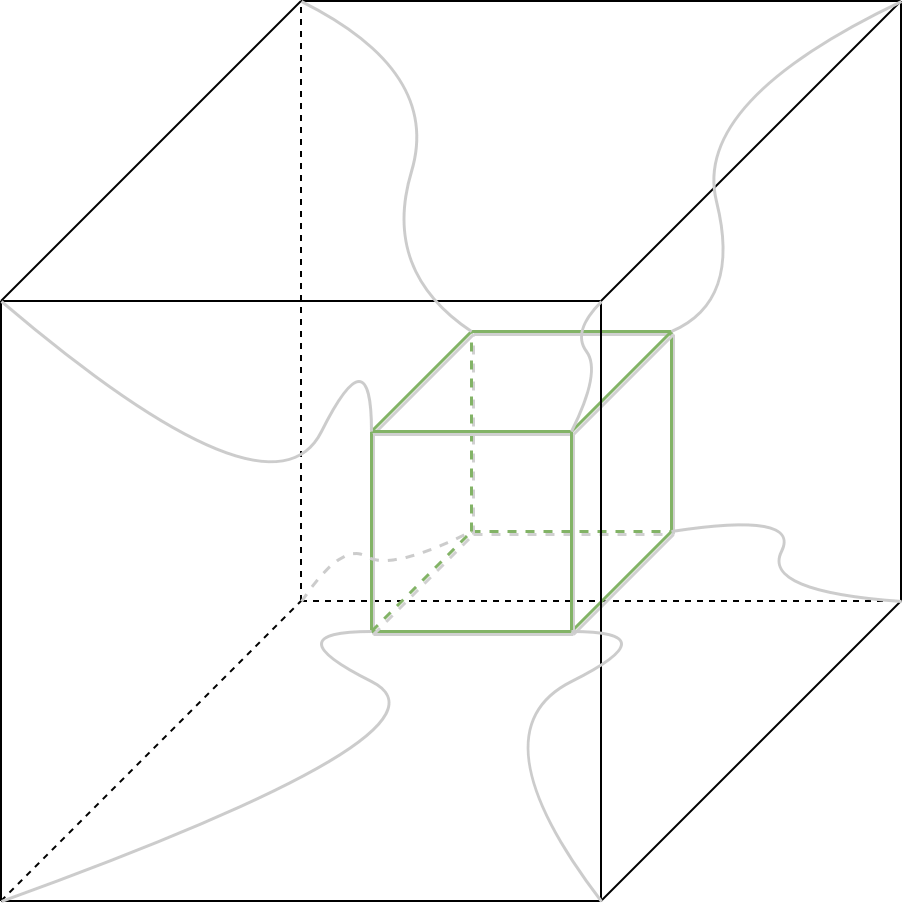
\includegraphics[width=8cm]{cube4d}
\end{center}
\caption{$W_4$}
\label{fig:2.b}
\end{figure}

\subtask{c}
Alle Punkte mit einer Koordinate $<0$ liegen außerhalb des Simplex. Im positiven Sektor wird das Simplex begrenzt durch eine Hyperebene. Der Bereich der von den Koordinatenachsen und dieser Hyperebene eingeschlossen wird ist genau das Simplex. Die Ecken des Simplex sind somit stets $0^d$ und die $d$ vielen Ecken die benötigt werden, um die Hyperebene zu definieren (das sind genau die Ecken $(1,0,...,0),...,(0,...0,1)$). Es gibt also $d+1$ viele Ecken.

Offenbar entstehen so stets $d+1$ viele Facetten (der ''Boden'' und $d$ viele, die inzident zu $0^d$ sind). Die Ecken, welche die Hyperebene beschreiben, sind zwar paarweise adjazent, liegen jedoch alle auf besagter Hyperebene, weshalb keine zusätzlichen Facetten entstehen. Für $S_4$ (siehe auch Abb. \ref{fig:2.c}) liegt beispielsweise $p_4$ auf der selben Facette wie $p_1,...,p_3$.

\begin{figure}[h!]
\begin{center}
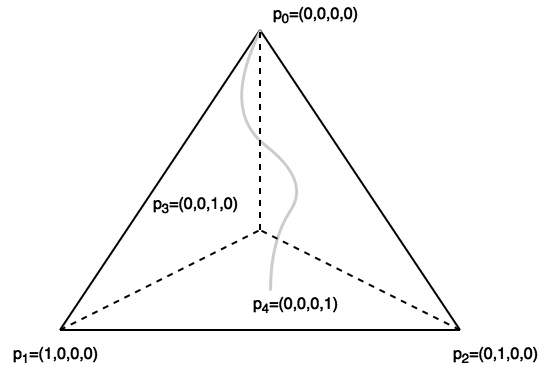
\includegraphics[width=8cm]{simplex4d}
\end{center}
\caption{$S_4$ - man sieht deutlich 5 Facetten :)}
\label{fig:2.c}
\end{figure}
\end{task}

\begin{task}{Konvexe Hülle}
\item[]
Punkte einen nach dem anderen hinzuzufügen und konvexe Hülle aktualisieren klingt gut: Wenn der hinzukommende Punkt innerhalb bzw. auf dem Rand der kovexen Hülle liegt, dann muss man nichts tun, nur wenn er außerhalb liegt wird es interessant.

Von dem Punkt aus gesehen, würde ich das Ding in die Ebene projizieren. Flächen einfügen zwischen allen Kanten die auf dem entstanden Rand liegen und dem Punkt. Kanten zwischen allen Knoten auf Rand und Punkt hinzufügen

Der ganze Rest der nun verdeckt wird wegschmeißen.
\end{task}
\end{document}